\section{Introduzione}

I sistemi per l'analisi microfluidica implementano soluzioni tecnologiche per contare, intrappolare, focalizzare, separare e identificare le proprietà della cellula. 

Possono essere identificate le proprietà di singole cellule basandosi su differenze nelle dimensioni e nelle proprietà dielettriche, sfruttando tecniche non invasive e senza richiedere l'ausilio di labelling cellulare.

Tra le differenti tecniche risalta l'analisi di impedenza in microfluidica. Si utilizzano più coppie di elettrodi, poste intorno al canale microfluidico, per applicare una tensione a frequenze discrete e misurare le fluttuazioni della corrente elettrica. Tali fluttuazioni sono dovute al passaggio della cellula all'interno del canale e quindi all'interno del campo elettrico non uniforme generato dagli elettrodi. 

Tali sistemi possono essere più o meno accurati a seconda della configurazione utilizzata.

In questo report viene presentata l'analisi di una tecnica di compensazione per eliminare la dipendenza dalla posizione nel canale che affligge i segnali misurati e non permette una corretta stima del diametro cellulare.

Tale tecnica di compensazione sfrutta la dipendenza del diametro elettrico dal parametro di forma, legato alle proprietà del segnale misurato. Nonostante le diverse famiglie analizzate (differenti diametri) appaiono come segnali non distinguibili il mapping mediante tale procedura di compensazione permette di produrre dei segnali dove le diverse famiglie sono chiaramente distinguibili.

\section{Background}

\begin{figure*}
	\begin{subfigure}{0.6\linewidth}
		\centering
		\footnotesize{ \def\svgwidth{\linewidth}
	    \input{channel_draw.pdf_tex}}
		\caption{}
	\end{subfigure}\hfill
	\begin{subfigure}{0.4\linewidth}
	\centering
	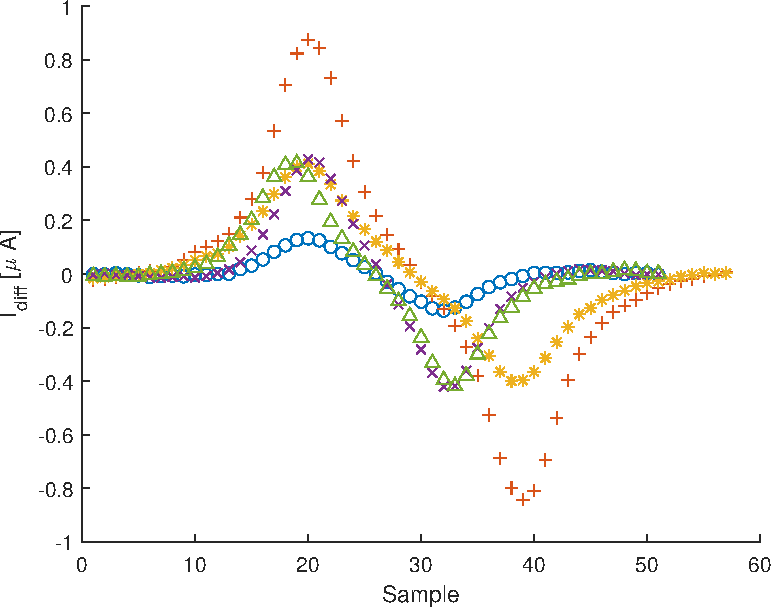
\includegraphics[width=.95\linewidth]{signal_visualization_fig.pdf}
	\caption{}
\end{subfigure}
\caption{Schema rappresentativo del citometro ad impedenza con la configurazione di elettrodi selezionata e la cellula passante (a); segnali della corrente differenziale misurata per 5 diversi campioni (b)}
\label{fig:generale}
\end{figure*}

Il citometro ad impedenza è un dispositivo microfluidico utilizzato per misurare le perturbazioni del campo elettrico all'interno di un microcanale dove passa una cellula. La cellula attraversa uno specifico pattern di elettrodi sul quale viene applicata un tensione alternata e questo porta ad una variazione della corrente misurata.

Ovvero si considera un microcanale riempito di un buffer conduttivo al cui interno passano delle correnti elettriche. Nel dispositivo in questione si applica un potenziale all'elettrodo centrale e si misura una corrente differenziale tra i due elettrodi laterali.

Si utilizzando basse frequenze per determinare le proprietà sulla dimensione della cellula in quanto il segnale è tipicamente proporzionale al volume cellulare. Alte frequenze, invece, vengono utilizzare per avere informazioni sulla conduttività della membrana cellulare.

Nel seguente report viene considerata una configurazione ad elettrodi coplanari rappresentata in \cref{fig:generale}.

Tramite la misura di corrente differenziale è possibile stimare alcune proprietà della cellula che passa nel canale. In particolare, al passaggio delle cellula, si misura un segnale con una forma d'onda di tipo gaussiana bipolare.

Tramite l'ampiezza di picco è possibile stimare il diametro elettrico. Il segnale è proporzionale al volume della cellula per cui il diametro sarà legato all'ampiezza del segnale ($a$) come:


\begin{equation}
	D=G a^{1 / 3}
\end{equation}

Dove $G$ è un guadagno che risente delle proprietà elettriche specifiche del dispositivo utilizzato.

\subsection{Gaussiana bipolare}

\begin{figure}[b!]
		\centering
		\footnotesize{ \def\svgwidth{0.95\linewidth}
			\input{bipolarGaussian.pdf_tex}}
	\caption{Forma d'onda di tipo gaussiana bipolare identificata dall'ampiezza $a$, punto centrare $t_c$, larghezza a metà altezza $2\sigma$ e distanza picco-picco $\delta$.}
	\label{fig:gaussiana}
\end{figure}


La gaussiana bipolare è una forma d'onda caratteristica composta da due gaussiane identificata dalla generica equazione:

\begin{equation}
	g(t)=a\left[e^{g_{+}(t)}-e^{g_{-}(t)}\right]
	\label{eq:gaussianabipolare}
\end{equation}

Ovvero, considerata un'ampiezza di riferimento $a$ (i.e. il valore massimo di picco), la forma d'onda complessiva è data dalla somma di due gaussiane nel tempo di cui la seconda ribaltata. 

La distanza picco-picco è pari a $\delta$ e si introduce un parametro di centratura $t_c$. 

Le due gaussiane condividono la medesima deviazione standard $\sigma$ e sono identificate dalle \cref{eq:gaussiana1} e \cref{eq:gaussiana2}.

\begin{equation}
	g_{+}(t)=\frac{-\left(t-\left(t_{c} +(\delta / 2)\right)\right)^{2}}{2 \sigma^{2}}
	\label{eq:gaussiana1}
\end{equation}



\begin{equation}
	g_{-}(t)=\frac{-\left(t-\left(t_{c} -(\delta / 2)\right)\right)^{2}}{2 \sigma^{2}}
		\label{eq:gaussiana2}
\end{equation} 

\subsection{Procedura di fitting}

Partendo dai dati sperimentali è necessario introdurre una procedura di fitting numerico per identificare la gaussiana, e quindi i suoi quattro parametri descrittivi, tale da rappresentare il segnale analizzato \cite{caselli_simple_2016}.

Tale procedura di fitting viene implementata secondo un algoritmo di ottimizzazione. Ovvero, si cerca di ridurre la differenza tra il dato misurato $[d]_i$ e il template di fitting $g(t_i)$ allo stesso instante temporale. 

Definita la funzione di errore come tale differenza:

\begin{equation}
	\underline{e}=[d]_{i}-g_{i}\left(t_{i}, a,t_c,\delta,\sigma\right)
\end{equation}

Si cerca di minimizzare la funzione obiettivo definita proprio come la norma dell'errore:

\begin{equation}
	\mathrm{E}(a,t_c,\delta,\sigma) = \frac{1}{2} \sum_{i}\left\|d_{i}-g\left(t_{i},a,t_c,\delta,\sigma\right)\right\|^{2}
\end{equation}


\subsection{Accuratezza}


I dispositivi microfluidi possono essere più o meno accurati. Questo è legato alla configurazione degli elettrodi, alla geometria, al mezzo di sospensione e velocità del flusso \cite{sun_single-cell_2010}.

In particolare, per il caso di riferimento si osserva una dipendenza del segnale dalla posizione all'interno del canale. Nonostante l'ampiezza del picco della gaussiana sia correlata con il diametro cellulare si osserva una dipendenza anche dalla posizione.

Ovvero, a parità di diametro, una cellula passante vicino agli elettrodi darà un picco di ampiezza maggiore alla stessa cellula passante ad una distanza maggiore \cite{spencer_high_2016}.

Nonostante nella configurazione utilizzata non si può avere una misura diretta della posizione all'interno del canale è possibile ottenerne una stima effettuando una compensazione del segnale tenendo conto della correlazione tra la posizione e lo shape parameters.

In particolare, risulta valida la relazione tra il parametro di forma $\mathtt{shape}$ e il diametro normalizzato che segue una legge lineare:
\begin{equation}
	{D\over d}={c_1+c_2\left(\sigma \over \delta \right)}
	\label{eq:compensazione}
\end{equation}

Dove:

\begin{equation}
	{\sigma \over \delta} = \mathtt{shape}
\end{equation}

Si possono quindi usare tali coefficienti della retta, calcolati per ogni segnale, per correggere il diametro elettrico rimuovendo l'effetto di posizione \cite{errico_mitigating_2017}.


%\begin{figure}[t!]
%	\centering
%	\includegraphics[width=0.95\linewidth]{imagefile}
%	\caption{}
%	\label{fig:}
%\end{figure}

\begin{figure}[t!]
	\centering
	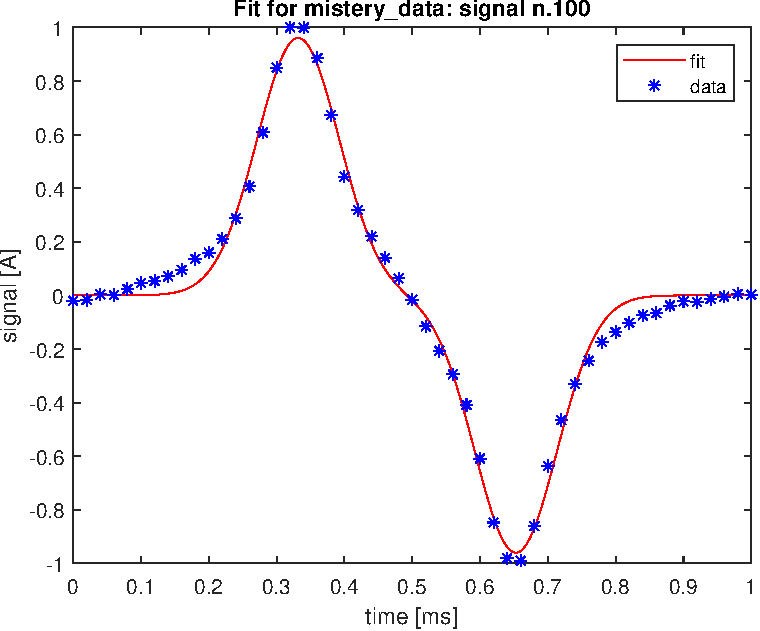
\includegraphics[width=0.9\linewidth]{fitted}
	\caption{Grafico dell'andamento temporale del segnale n. 100. In blu i campioni e in rosso il segnale fittato con una gaussiana bipolare}
	\label{fig:fitted}
\end{figure}




\subsection{Dataset di riferimento}

Il dataset di riferimento è un insieme di dati grezzi ottenuti da misurazioni di citometria ad impedenza su un campione di biglie di test. 

Sono presenti i segnali di tre famiglie di biglie di test con diametro nominale di $5.2,\:6\text{ e }7 \mu m$. 

Per il dispositivo in questione il guadagno è pari a 10.5 $\mu$m / A\textsuperscript{1/3} e la distanza inter-elettrodo è pari a $L=40\: \mu m$. 

I segnali sono campionati con una frequenza $f_s=115$ kHz con un totale di oltre 50.000 segnali.



\section{Risultati}

Inizialmente la procedura viene applicata su un dataset ristretto considerando solamente 400 segnali. Vengono selezionati quindi i segnali di indice da 400 a 800.

Successivamente la procedura verrà applicata anche su un riferimento più esteso.

\subsection{Fitting numerico}

A partire dal singolo segnale all'interno dell'intero dataset è possibile fittare la gaussiana bipolare andando a stimarne i quattro coefficienti descrittivi.

Considerando il template in \cref{eq:gaussianabipolare} è possibile utilizzare il comando Matlab \texttt{fit()} fornendo il template stesso, i dati e i valori iniziali per la stima ai minimi quadrati.

Inoltre, essendo il segnale molto piccolo $\propto 10^{-6}$ è utile normalizzare il segnale di ampiezza e scalare l'asse dei tempi riportandolo in secondi nel range $[0;\:{1\over f_s}]$ con un numero di campioni equivalente, dove $f_s$ è la frequenza di campionamento il cui inverso indica l'ultimo campione temporale.

A questo deve seguire poi necessariamente una riscalatura nel dominio originario per poter confrontare i segnali ed effettuare la procedura di compensazione correttamente.

Un esempio di fitting è presente in \cref{fig:fitted} ed è evidente come la gaussiana bipolare sia descrittiva del segnale misurato.

\begin{figure}[t!]
	\centering
	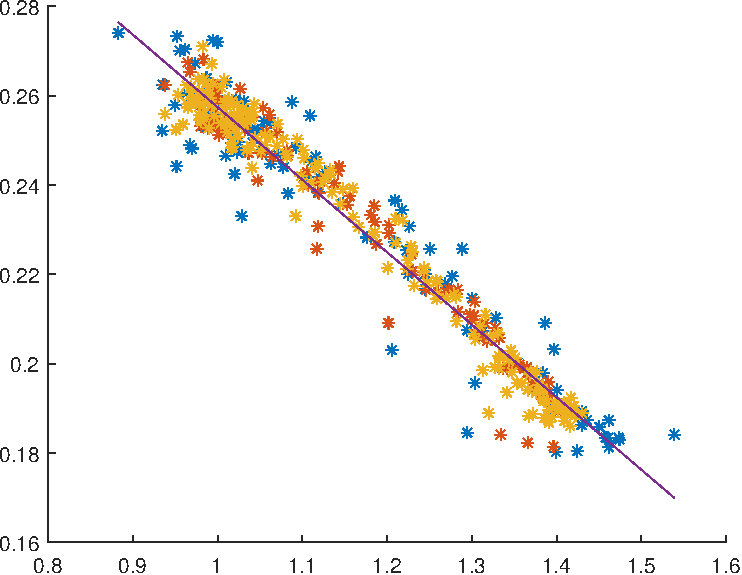
\includegraphics[width=0.9\linewidth]{normalized_diam_figs}
	\caption{Andamento dello shape parameter rispetto il diametro normalizzato. Sono raffigurati i campioni delle tre famiglie distinte con colori differenti e la retta ottenuta con una procedura di fitting lineare.}
	\label{fig:normalized}
\end{figure}

\begin{figure*}[t!]
	\centering
	\begin{subfigure}{0.5\linewidth}
		\centering
		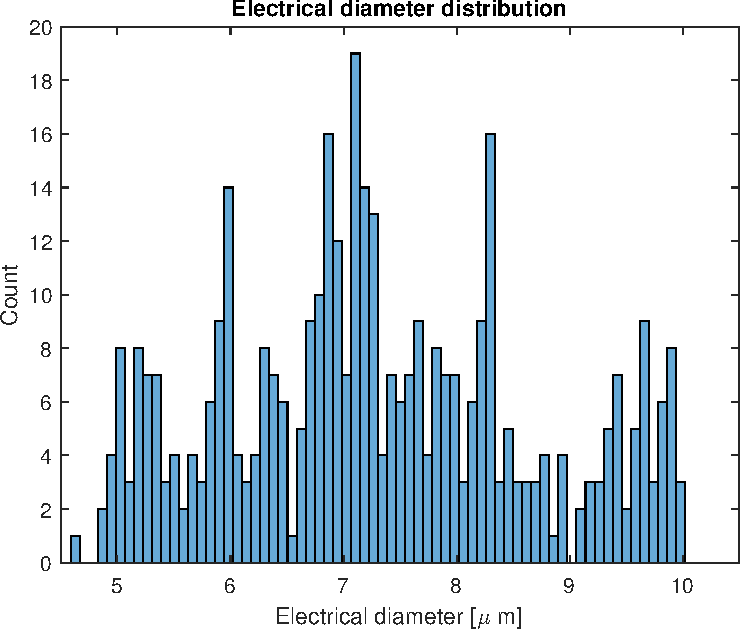
\includegraphics[width=0.8\linewidth]{histogram_figs}
		\caption{}
		\label{fig:histo}
	\end{subfigure}\hfill
	\begin{subfigure}{0.5\linewidth}
		\centering
		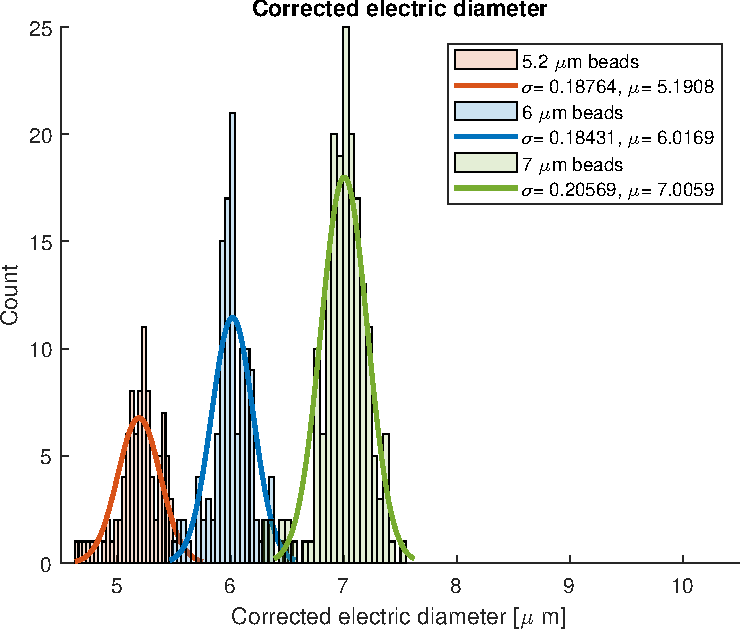
\includegraphics[width=0.8\linewidth]{histogram_corrected2_fig}
		\caption{}
	\end{subfigure}
	\caption{Distribuzione dei diametri elettrici rappresentata con un istogramma prima della correzione (a) e dopo la procedura di compensazione (b). Sono evidenti le tre famiglie distinte dopo la procedura di compensazione.}
	\label{fig:histogram}
	\vspace{0.5cm}
	\centering
	\begin{subfigure}{0.5\linewidth}
		\centering
		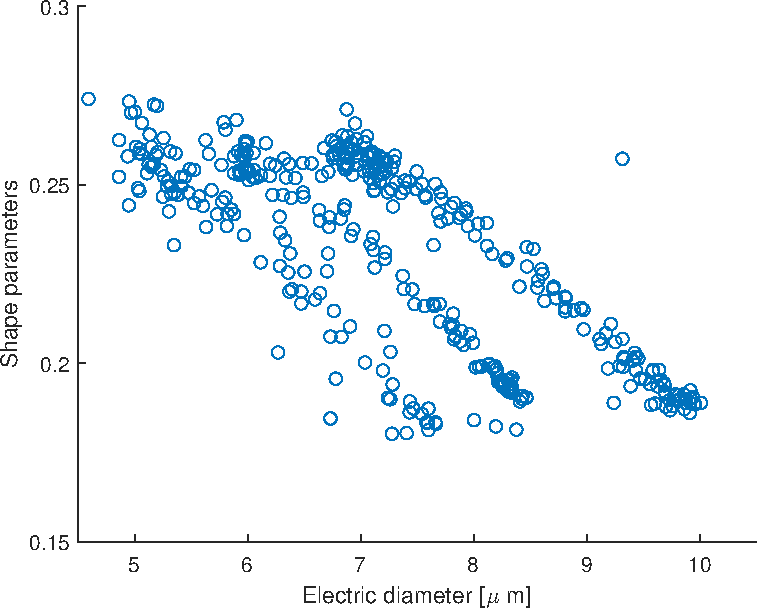
\includegraphics[width=0.8\linewidth]{scatter_fig}
		\caption{}
		\label{fig:scatter_init}
	\end{subfigure}\hfill
	\begin{subfigure}{0.5\linewidth}
		\centering
		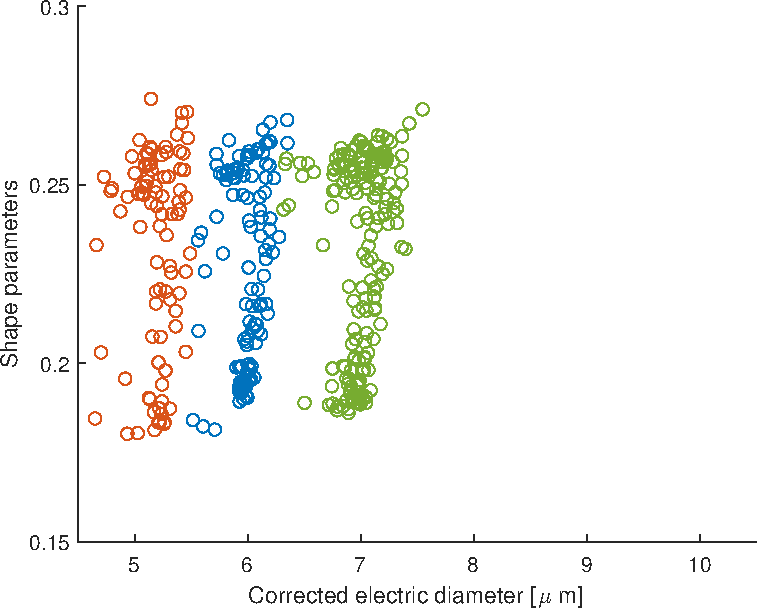
\includegraphics[width=0.8\linewidth]{scatter_corrected2_fig}
		\caption{}
	\end{subfigure}
	\caption{Scatter plot dello shape parameter rispetto al diametro elettrico prima (a) e dopo (b) la compensazione. La procedura di compensazione porta ad una netta distinzione delle tre famiglie. Si passa da tre bande diagonali, dove è impossibile stabilire il diametro senza portare in conto l'incertezza del contributo posizionale, a tre bande verticali che chiaramente separano le tre differenti famiglie. }
	\label{fig:scatter}
		\vspace{0.5cm}
	\centering
	\begin{subfigure}{0.5\linewidth}
		\centering
		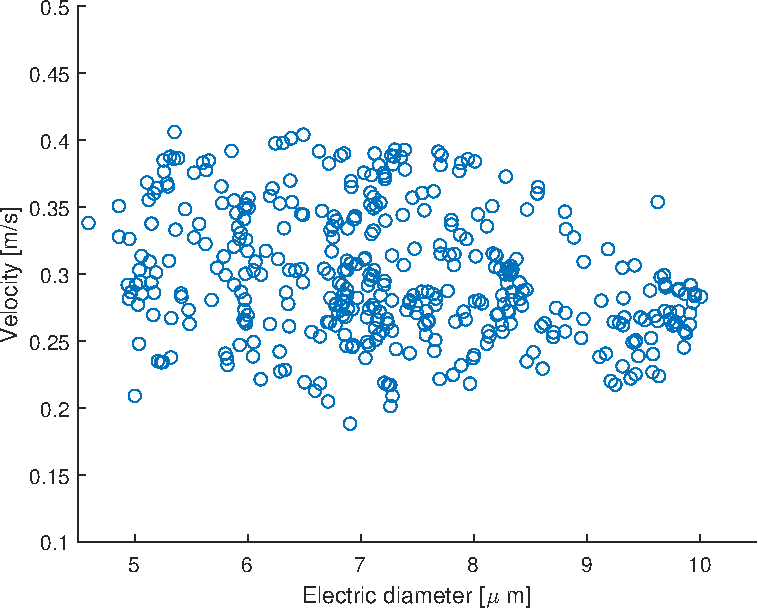
\includegraphics[width=0.8\linewidth]{velocity_fig}
		\caption{}
	\end{subfigure}\hfill
	\begin{subfigure}{0.5\linewidth}
		\centering
		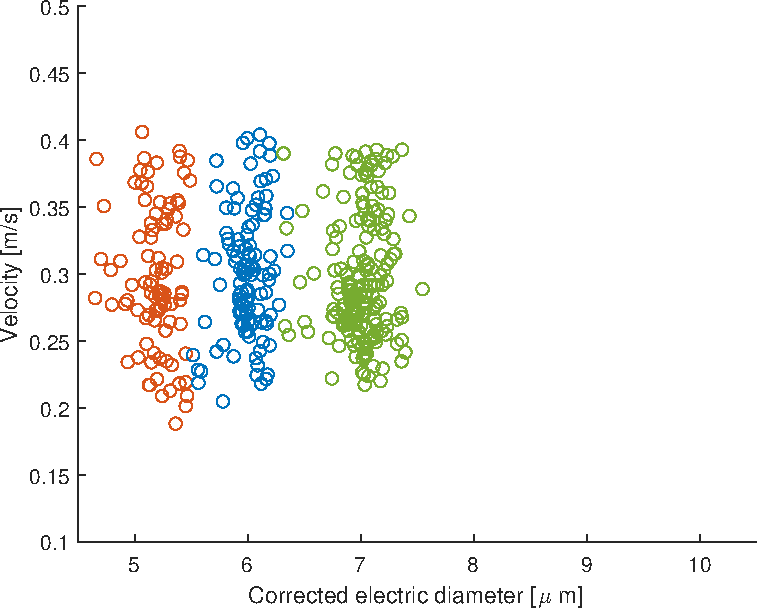
\includegraphics[width=0.8\linewidth]{velocity_corrected_fig}
		\caption{}
	\end{subfigure}
	\caption{Scatter plot della velocità rispetto al diametro elettrico prima (a) e dopo (b) la compensazione. Si vede come la procedura di compensazione porta ad una netta distinzione delle tre famiglie che nel caso pre-compensazione non era presente.}
	\label{fig:velocity}
\end{figure*}


\subsection{Compensazione}


\begin{figure*}[h!]
	\centering
	\begin{subfigure}{0.33\linewidth}
		\centering
		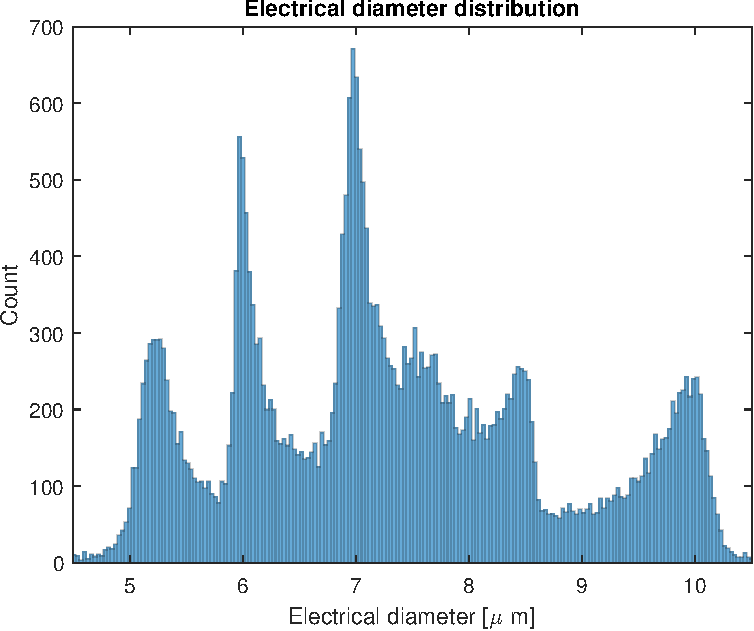
\includegraphics[width=0.9\linewidth]{histogram_data}
		\caption{}
	\end{subfigure}\hfill
	\begin{subfigure}{0.33\linewidth}
		\centering
		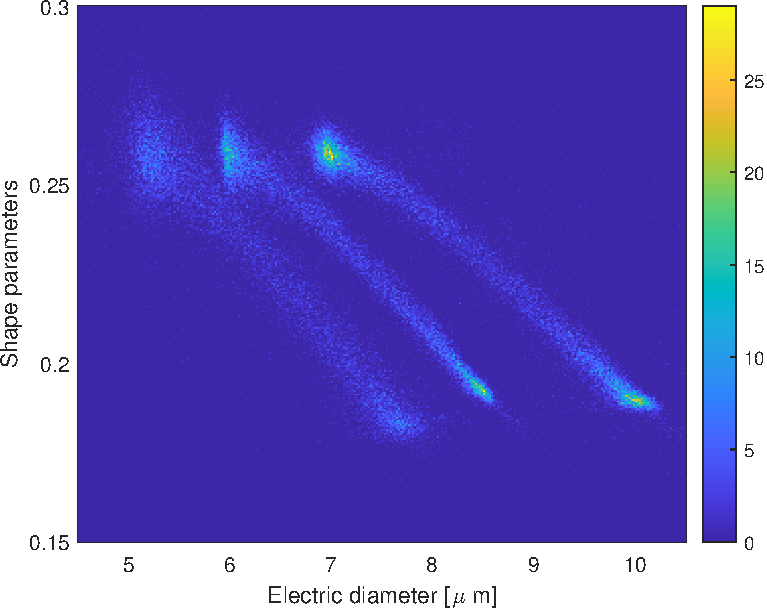
\includegraphics[width=0.9\linewidth]{density_diam_shape}
		\caption{}
	\end{subfigure}\hfill
	\begin{subfigure}{0.33\linewidth}
		\centering
		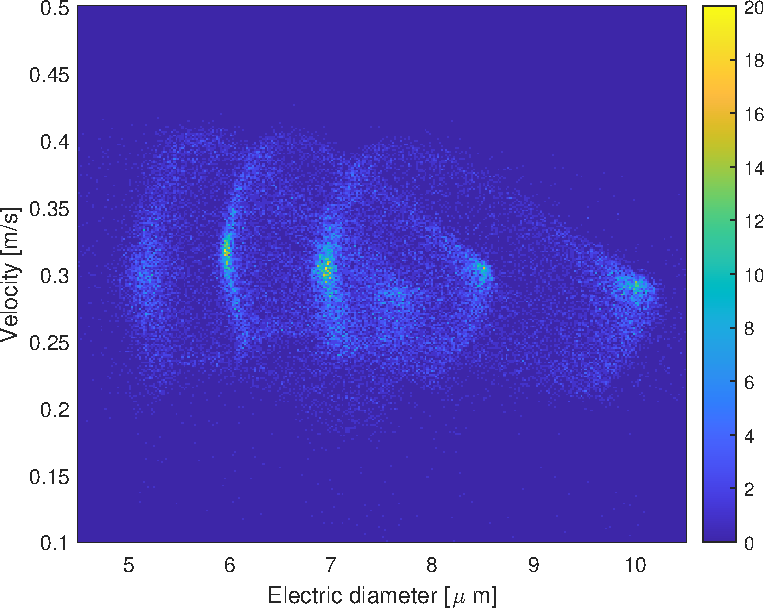
\includegraphics[width=0.9\linewidth]{density_diam_velocity}
		\caption{}
	\end{subfigure}\hfill
	\begin{subfigure}{0.33\linewidth}
		\centering
		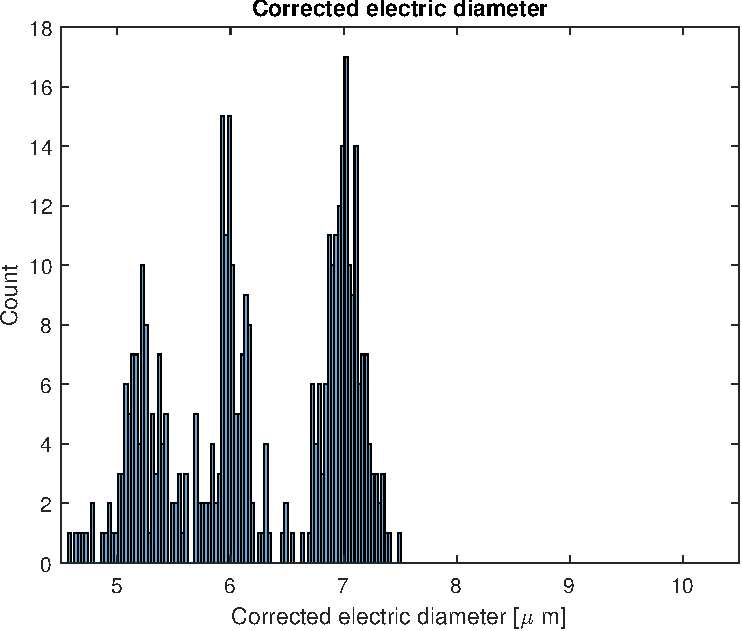
\includegraphics[width=0.9\linewidth]{histogram_corrected_fig}
		\caption{}
		\label{fig:hist_Sep}
	\end{subfigure}\hfill
	\begin{subfigure}{0.33\linewidth}
		\centering
		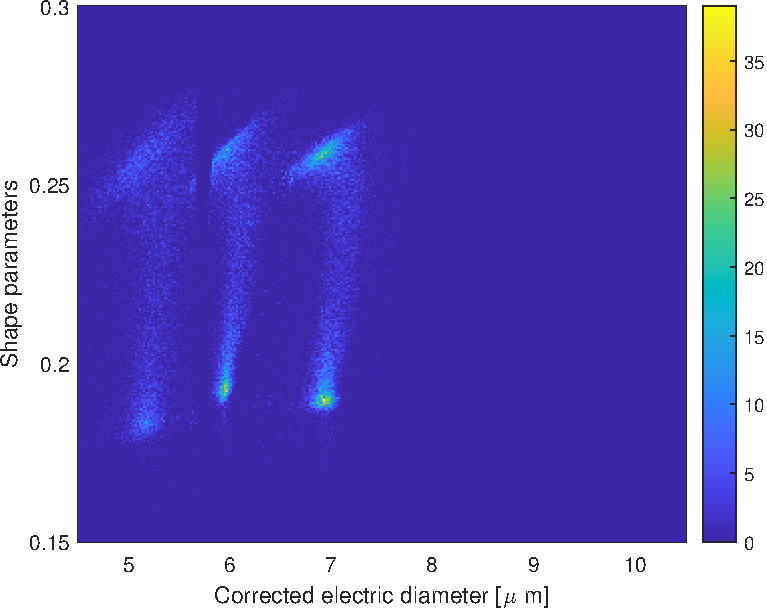
\includegraphics[width=0.9\linewidth]{density_diam_corr_shape}
		\caption{}
	\end{subfigure}\hfill
	\begin{subfigure}{0.33\linewidth}
		\centering
		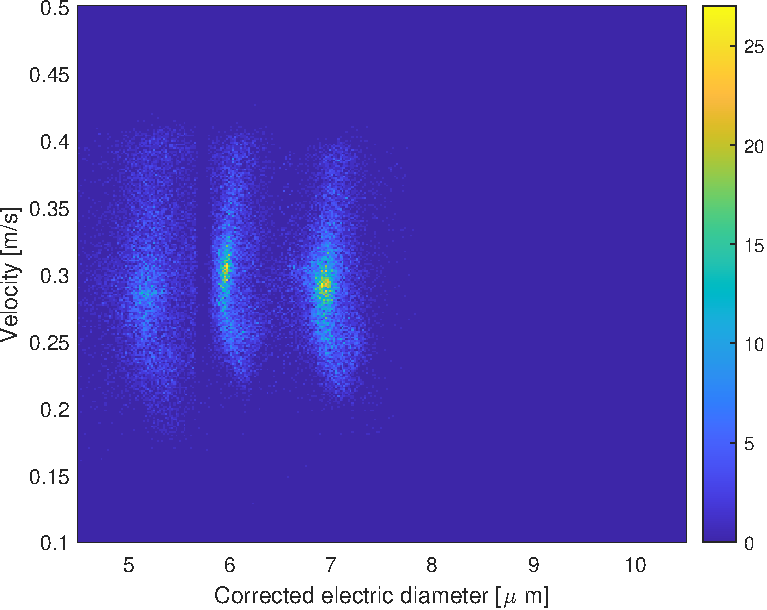
\includegraphics[width=0.9\linewidth]{density_diam_corr_velocity}
		\caption{}
	\end{subfigure}
	\caption{Analisi su 35000 campioni. Viene nuovamente applicata la procedura di test ma su un numero di segnali maggiori la cui distribuzione è presentata tramite istogramma (a). Considerando molti segnali risultano statisticamente evidenti i picchi relativi alle tre famiglie ma non è possibile distinguere nettamente i segnali. La distinzione invece appare netta ed evidente dopo la compensazione (d). Sono riportati anche i plot di densità per lo shape parameters rispetto al diametro elettrico prima (b) e dopo (e) la compensazione e per la velocità rispetto al diametro elettrico prima (c) e dopo (f) la compensazione. Dai diagrammi di densità risulta evidente la netta separazione che viene segue alla procedura di compensazione. }
	\label{fig:density}
\end{figure*}


Per la procedura di compensazione è necessario stimare i coefficienti della retta derivante dal fitting lineare. 

Tale fitting deve essere fatto nello spazio $[{\delta\over \sigma};\:{D\over d}$] ed è quindi necessario normalizzare i diametri elettrici rispetto i singoli diametri nominali delle tre famiglie. 

Bensì in questo dataset non sia possibile identificare a priori, con una procedura automatica, la famiglia di appartenenza della misura si può sfruttare lo scatter plot del diametro elettrico vs shape parameters per distinguere visivamente tre famiglie (\cref{fig:scatter_init}). Quindi, mediante la funzione \texttt{inpolygon()} è possibile selezionare manualmente i valori corrispondenti alle tre famiglie, separarle e quindi normalizzarle per il rispettivo diametro nominale. 

Quindi è possibile calcolare la retta che meglio approssima l'andamento dello shape parameter in funzione del diametro elettrico normalizzato (\cref{fig:normalized}). Dunque è possibile estrarre i coefficienti:
\begin{itemize}
	\item $\mathtt{c1}=2.59$
	\item $\mathtt{c2}=-6.20$
\end{itemize}

All'interno dell'ambiente Matlab è possibile utilizzare il comando \texttt{fitlm()} così da ottenere direttamente i due coefficienti della retta e anche una stima del coefficiente di determinazione $\mathtt{r}^2=0.96$. 

Tramite tali coefficienti è possibile correggere i valori tramite l'\cref{eq:compensazione}.

Si ottengono quindi le famiglie separate sia nello scatter plot dello shape parameter che della velocità, in \cref{fig:scatter} e \cref{fig:velocity}.

\begin{table}[b!]
	\centering
	\begin{tabular}{|c|p{ 1.5 cm}|c|p{1.9 cm}|p{ 1.4 cm}|}
		\hline
		& \footnotesize{Deviazione standard} & \footnotesize{Media} & \footnotesize{Coefficiente di variazione} & \footnotesize{Diametro nominale} \\
		\hline
		\# 1 & 0.187 & 5.196 & 0.035 & 5.2 $\mu m$ \\
		\hline
		\# 2 & 0.184 & 6.016 & 0.031 & 6 $\mu m$\\
		\hline
		\# 3 & 0.205 & 7.005 & 0.029 & 7 $\mu m$\\
		\hline
	\end{tabular}
	\caption{Coefficienti della distribuzione gaussiana per le tre famiglie ottenuti dal fitting dei valori dell'istogramma}
	\label{tab:fithist}
\end{table}

\subsection{Distribuzioni}

Chiaramente tale procedura, separando le famiglie, permette il calcolo della loro distribuzione.

Analizzando la distribuzione dei segnali, prima della compensazione, è evidente come non sia possibile identificare alcun picco nel grafico dell'istogramma in \cref{fig:histo}. 
Questo grafico è pienamente rappresentativo di come i segnali siano effettivamente mischiati a causa del contributo di posizione.

Dopo la compensazione, invece, è chiaramente possibile distinguere le diverse famiglie come è evidente dai tre picchi nettamente distinguibili in \cref{fig:histogram}.

Vengono riportate quindi le distribuzioni delle tra famiglie ciascuna con un andamento a gaussiana in cui parametri sono presenti in \cref{tab:fithist}. Risulta evidente come la maggioranza delle biglie rientrano nella terza famiglia, a diametro maggiore, ma tale valore rispecchia anche una maggiore dispersività. Le due famiglie a dietro più piccolo presentano invece una dispersione confrontabile.



\begin{figure}[b!]
	\centering
	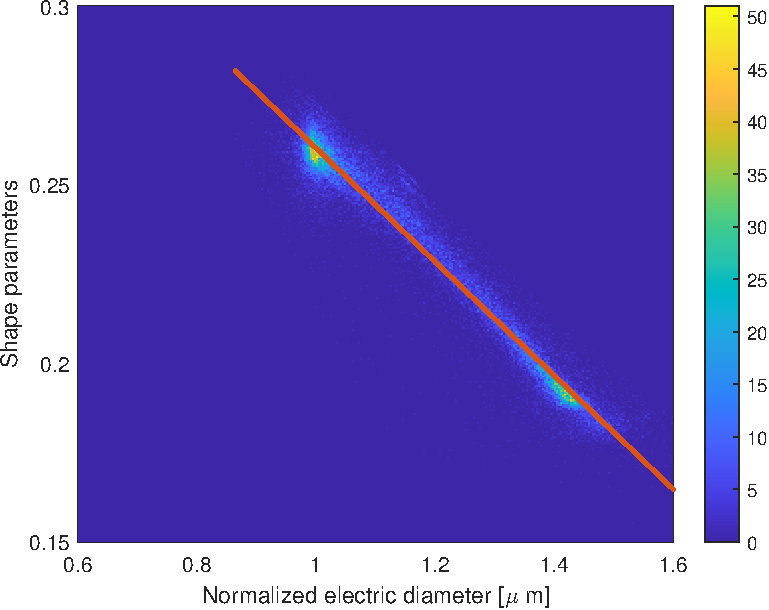
\includegraphics[width=0.9\linewidth]{normalized_D}
	\caption{Grafico di densità della distribuzione dei segnali del parametro di forma rispetto al diametro normalizzato. Sono presenti i dati di tutte e tre le famiglie con la retta interpolante unica.}
	\label{fig:normalizedDensity}
\end{figure}





\subsection{Estensione del dominio di interesse}




La stessa procedura può essere applicata anche su una quantità di segnali notevolmente maggiore. Vengono quindi considerati, nello stesso dataset di riferimento, i segnali di indice a 200 a 35200. 

La procedura può essere applicata allo stesso modo ma gli scatter plot vengono sostituiti da plot di densità che permettono di osservare meglio la distribuzione dei valori (\cref{fig:density}).

Nuovamente si ottengono i due parametri di fitting $c_1=2.63$, $c_2=-6.28$ tramite i quali applicare la procedura di compensazione.

In modo analogo segue l'istogramma dove si separano le tre famiglie (\cref{fig:hist_Sep}). In questo caso la maggioranza delle biglie rientrano comunque nella famiglia con diametro maggiore ma la famiglia con diametro più piccolo presenta una maggiore dispersione. 



\section{Conclusioni}

La procedura di compensazione permette di separare le differenti famiglie rispetto al diametro elettrico e risulta affidabile sia su pochi segnali che su campioni più vasti.

Tale procedura richiede di conoscere preventivamente i diametri delle biglie. 

Nel caso in cui i singoli segnali non siano associabili al relativo diametro nominale con certezza viene richiesta una procedura manuale di identificazione che, per sua natura, indurrà un certo errore nella classificazione e nel fitting lineare, quindi sulla procedura di compensazione. 

Tale errore si riflette principalmente in una dispersione nelle distribuzioni delle biglie. La deviazione standard delle distribuzioni delle famiglie rimane sotto lo 0.23 e macroscopicamente rimangono fortemente distinguibili le tre famiglie e le loro distribuzioni. 

Chiaramente, a causa dell'errore numerico presente e della grande quantità di outliers, non è facile classificare il singolo segnale quanto classificare la distribuzione macroscopica.

\raggedbottom
\pagebreak
\section*{Disponibilità dei dati}

Il materiale è disponibile alla repository online del progetto: \url{https://github.com/mastroalex/curve-fitting}


\raggedbottom
%\pagebreak
\printbibliography[title=Riferimenti]
%\section*{References}


%\clearpage
%\onecolumn
%\section*{Appendice}




